\section{Theorie}
\label{sec:Theorie}
Aufgrund der hohen Präzision werden üblicherwiese Brückenschaltungen eingesetzt. Um die Präzision zu gewährleisten wird die sogenannte Nullmethode eingesetzt.
Mit Hilfe dieser Methode werden die Schaltungen abgeglichen, damit die zu messenden Größen mit einer hohen Genauigkeit bestimmt werden können. Außerdem lässt sich jede
physikalische Größem, welche sich als elektrischer Widerstand darstellen lässt, sehr präzise messen.
\subsection{Allgmeine Brückenschaltung}
Um die Ableichbedigung zu berechnen, betrachtet man zunächst die Spannung zwischen zwei Punkten auf zwei verschieden Leitern. Die dort anliegende Potentialdifferenz U
zwischen den Punkten A und B, welche auch als Brückenspannung bezeichnet wird hängt von den Widerstandsverhältnissen ab,
weswegen man dieses Verhätnis zum Abgleichen ausnutzt.
Die allgemeine Gestalt einer Brückenschaltung wird in  Abbildung \ref{fig:allgBrücke}
\begin{figure}
    \centering
    \caption{Allgemeine Brückenschaltung} 
    \label{fig:allgBrücke}
    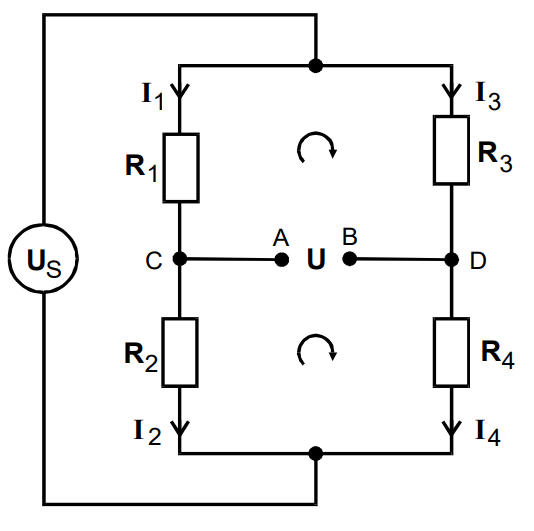
\includegraphics[width = 0.5\textwidth]{bridges/genbridge.png}
\end{figure}
dargestellt. Allgemein kann man Schaltkreise mit Hilfe der Kirchhoffschen Gesetzen beschreiben.
\subsection{Kirchoffschen Gesetze}
\subsubsection{Knotenregel}
Die erste Kirchhoffsche Regel ist die Knotenregel, welche besagt, dass die Summe der zufließenden Ströme gleich der Summe der abfließenden Ströme ist.
Mathematisch ausgedrückt sieht die Knotenregel wie foglt aus:
\begin{equation}
    \sum_{k=1}^N I_k = 0 \label{eqn:knotrule}
\end{equation} 
\begin{figure}
    \centering
    \caption{Illustration zur Knotenregel}
    \label{fig:knotrule}
    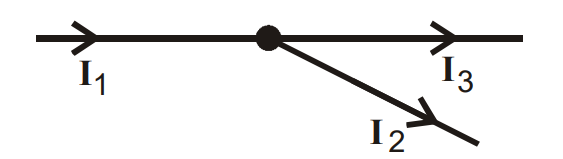
\includegraphics[width = 0.5\textwidth]{bridges/knotrule.png}
\end{figure}
Damit die Konfiguration in Abbildung \ref{fig:knotrule} gültig ist, müssen entweder die abfließenden Ströme $I_2$ und $I_3$ oder 
der zufließende Strom $I_1$ ein negatives Vorzeichen haben, so dass die Gleichung \eqref{eqn:knotrule} ihre Gültigkeit 
behält. Zwecks Konventionen besitzen die abfließenden Ströme negative Vorzeichen.
\subsubsection{Maschenregel}